\documentclass{article}
\usepackage[utf8]{inputenc}
\usepackage{fullpage}
\usepackage[backend=biber,style=apa,backref=true]{biblatex}
\usepackage{listings}
\lstset{language=tex}
\usepackage{url}
\usepackage{graphicx}
\graphicspath{./figs}
\usepackage{amsmath}
\usepackage{hyperref}
\hypersetup{colorlinks=true, citecolor=blue}

%for including wordcount in file
\immediate\write18{texcount -template="{word} words in main body, excluding headers and bibliography." \jobname.tex -out=\jobname.sum}
\usepackage{verbatim}
\newcommand\wordcount{\verbatiminput{\jobname.sum}}


\author{George Tyler}
\date{\today}

\addbibresource{diss.bib}
\begin{document}

\title{Social Media, Risk Perception, and Social Distancing: \\ Evidence from 33 Million Geolocated Tweets}

\maketitle
%This is a writing sample to be submitted to Economics Masters programmes. The writing sample will be assessed for a comprehensive understanding of the subject area; understanding of problems in the area; ability to construct and defend an argument; powers of analysis; and powers of expression. I should display the word count on the document. 
\abstract{Does social media predict risk-taking behaviour? I investigate this question in the context of COVID-19 by exploiting a large panel of tweets. Using inferred and explicit geolocation data embedded in the tweets, I study the extent to which public expressions of sentiment such as fear, anger, and optimism influence social distancing, as measured by GPS-located smartphone data. In this 2000-word excerpt, I motivate the research design and briefly describe the Twitter dataset.}

\section{Introduction}
\subsection{Overview}
The early stages of the COVID-19 pandemic saw an unprecedented shift in behaviour for most citizens of the United States. In a short period of time, a large number changed their habits of working, socialising, and travelling. They did so both as a result of government restrictions in the form of non-pharmaceutical interventions (NPIs) and as a private response to the spread of the pandemic. Economists have taken interest in how citizens formed these behaviour changes, and the role that beliefs and risk attitudes played in determining the response to public policy. A new way to measure belief formation and public sentiment is with social media, an increasingly common platform for expression of opinion. It is plausible that those who express more risk-averse sentiment towards COVID online will be inclined to respond in a stricter fashion to social distancing and other public health regulations. In this dissertation, I investigate the role of local expressions of risk attitude on public behaviour in the early months of the pandemic. Specifically, I study whether a measure of risk-averse sentiment on Twitter is linked to increased social distancing behaviour at the county/week level. 

This dissertation contributes to two strands of the recent economics literature on the COVID-19 pandemic. First, it investigates the relationship between partisanship and risk preference. Previous papers posit that political preference influences social distancing through risk preference; I contend that \textit{local} risk preference is a separate factor to political partisanship, and has an independent impact on social distancing. Second, this research relates to the recent economics literature around heterogeneous-agent epidemiological models, which endogenise individual behaviour -- including social distancing -- into the effective reproductive number \(R(t)\). These recent models, such as \textcite{acemogluTestingVoluntarySocial2020,brotherhoodEconomicModelCOVID192020,eichenbaumMacroeconomicsEpidemics2020}, assume that preferences over risk are predictive of social distancing behaviour; this paper looks to empirically confirm this key assumption. More broadly, the paper investigates the relationship between risk preference and economic behaviour, and presents a novel example of economic inference from social media using text analysis. 

A key vector for expressing sentiment is social media, with Twitter and Facebook's suite of products\footnote{Facebook, Facebook Messenger, Instagram, and WhatsApp} being the most widely-adopted, each platform having over 80 million monthly active users in the US. A survey by the Pew Research Foundation indicates that 22\% of US adults use Twitter, with 42\% of these using it on a daily basis \parencite{perrinShareAdultsUsing2019}. On Twitter, users can share their own text, with the option to link to a website; alternatively, they can `retweet' another user's text or link. Users can also use `hashtags' in their tweet, which connects their tweet to a particular topic. If the user has allowed it, Twitter also records the location of the tweet; and it is also possible for the user to set their location on their profile. In this way, it is possible to create a panel of geographically-located tweets about a particular topic. 

I exploit GeoCov19 \parencite{qaziGeoCoV19DatasetHundreds2020a}, a dataset of 524 million geolocated tweets, to measure the local public sentiment on COVID in the US. The tweets cover the period from 1st February to 1st May, the period I focus on. The particular subset of the data I use contains 33.36 million tweets in total; a small subset are exactly geolocated (the user has provided a GPS location), while most are inferred from the location tab in the user's profile. The tweets were collected using the Twitter Streaming API, querying for tweets containing any of a list of 800 COVID-related keywords. I also use anonymous smartphone location data, collected by the company SafeGraph, as a measure of the extent of social distancing in an area. I present two measures of social distancing at county level: first, the median minutes spent at home during 8am-6pm; second, the proportion of measured devices that stayed at home all day \parencite{safegraphinc.SocialDistancingMetrics2020}. Demographic controls are also acquired and presented from the American Community Survey and the 2010 US census. 

I use dictionary-based text analysis to assess the level of risk sentiment in a tweet. More sophisticated methods of text analysis like latent factor modelling are discussed in the Methods section. In the absence of a lexicon of risk preference, the NRC Emotion Lexicon \parencite{mohammadCrowdsourcingWordEmotion2013} is used. This is a widely-used mapping of English words to eight basic emotions (anger, fear, anticipation, trust, surprise, sadness, joy, and disgust). Starting from a set of tweets that mention COVID, I assign tweets containing fear-associated words to a risk-averse sentiment. The base unit of analysis is the county-week; as such, I measure the proportion of tweets that contain fearful language in each county and week. 

It is plausible that social media is a valid measure for risk appetite. The intuition is that the textual content of a social media post broadly reflects the poster's current opinion of a topic: for example, in response to the first confirmed US COVID death on February 26th, a user may express fearful, or uncertain, sentiment: for example, `i think i have 70 panic attacks every day because of how scared i am for my mom to catch corona', a Tweet in the dataset -- or a neutral sentiment. This opinion of the topic, particularly their level of fear, maps to a user's broader expectations about the course of the pandemic: while other emotions like joy, anticipation, and trust may rely on the context of the discussion, expressions of fear are plausibly consistent in mapping to risk-averse sentiment. When restrictions are implemented, users who initially formed pessimistic expectations may be more inclined to adhere more to them than a user who formed optimistic or netural expectations. 

The primary econometric specification is a panel model with county and week fixed effects;
\[Y_{it} = \alpha + \beta r_{it} + \mu c_{it} + \tau_i + \delta_t +  X_{it}\gamma + \epsilon_{it}\]
where \(Y_{it}\) is a vector of social distancing metrics, \(\beta r_{it}\) is the risk perception measure, (i.e. the proportion of total tweets containing fearful language), \(\mu c_{it}\) the number of COVID cases, \(\tau_i + \delta_t\) county and week-level fixed effects, and \(X_{it}\gamma\) demographic controls.



This research contributes to the recent economics literature seeking to explain the disparities in social distancing in the early stages of the pandemic in the US. In particular, partisanship has been shown to be a significant factor on the practice of social distancing: \textcite{allcottPolarizationPublicHealth2020,barriosRiskPerceptionLens2020,painterPoliticalBeliefsAffect2020} show that areas with more Republicans engaged in less social distancing, are associated with lower perceptions of risk of the pandemic, and exhibited less remote transactions. \textcite{simonovPersuasiveEffectFox2020,ananyevSafestTimeFly2020} also measure the causal effect of the right-wing Fox News network on social distancing during the pandemic. This paper builds on \textcite{barriosRiskPerceptionLens2020} in particular, which shows that online risk perception is predicted by Trump voter share: by measuring risk perception with a high-frequency geolocated dataset, my approach controls for political alignment and assesses the effect of risk perceptions on their own. In essence, the above papers argue that political beliefs affect complicance with Social Distancing orders; I measure expressions of sentiment regarding COVID risk, and given this data I ask two questions: first, does local risk sentiment predict social distancing behaviour beyond political affilitation; second, do differing interpretations of political messages -- like Trump's messages in March and April downplaying the virus -- colour local risk sentiment?


This dissertation also contributes to the rapidly-expanding field of text analysis in economics, and presents an example of how the rich sentiment data encoded in social media communication can inform insights into public behaviour. This topic is particularly mature in finance -- where sentiment data from public company documents, news media, and social media have been shown to predict stock market reactions \parencite{bollenTwitterMoodPredicts2011} -- and monetary economics, where central bank statements, coded according to their dovishness or hawkishness, predict fluctuations in Treasury securities \parencite{luccaMeasuringCentralBank2009,gentzkowTextData2019}. On the topic of empirical economics, this paper takes a similar approach -- by using online data to predict local sentiment -- as \textcite{stephens-davidowitzCostRacialAnimus2014}, which uses Google search data to proxy an area's racial animus, and uses this to estimate the Obama vote share. I use geolocated Twitter sentiment to proxy the local attitude to COVID in a given week, and test to see if this predicts social distancing practice. 

The argument of the dissertation rests on the following assumptions: first, that social media data is a valid proxy for local risk appetite, and that fear-associated language in COVID-related tweets is an effective estimator of the risk appetite encoded in the tweet. It is also important to note a possible selection effect in the dataset: tweets about COVID may attract a greater level of fear-related language and not reflect an individual's true opinion about social distancing and other preventative measures. I address these assumptions and drawbacks and discuss methods to alleviate them in the Results section.


\section{Literature Review}%Aim: 3000 words
\subsection{Text analysis in Economics}
\subsection{Digital trace datasets and social media}
\subsection{COVID-19 policies and social distancing}

\section{Data} %2000-3000 words
\subsection{GeoCoV19 and geolocation inference of Twitter datasets}
The primary dataset of tweets I present is a subset of GeoCoV19, a project which collected tweets relating to COVID-19 between February 1 and May 1 2020. The Twitter Streaming API provides a live filter function for a number of keywords and hashtags, and returns all tweets matching any of the search terms. The terms were chosen to cover a broad base of COVID-related talk, including searches for symptoms (e.g.`breathing difficulties'), behaviour (e.g. `\#masks4all'), and popular hashtags (e.g. `\#IStayHome, \#FlattenTheCurve') in addition to central discussion topics like `coronavirus'. The full list of search terms used is in a separate appendix. The dataset was collected with multilingual use in mind, but a majority of the tweets were based in the US; tracking with the fact that the US makes up most of Twitter's user base. In total, 524 million tweets were collected during the time period; during the first three weeks of February this number was lower, reflecting lower general interest, and increasing to around 6.4 million per day during March and April. We filter for tweets that are in English and are geotagged to originate from the United States. This primary dataset is supplemented with exact-geolocation Tweets from two other similar datasets, \textcite{bandaLargescaleCOVID19Twitter2021,lamsalDesignAnalysisLargescale2020}. The collection method for both datasets is broadly similar to GeoCoV19, using the Streaming API and a set of COVID-related keywords. 
\begin{figure}[h!]
    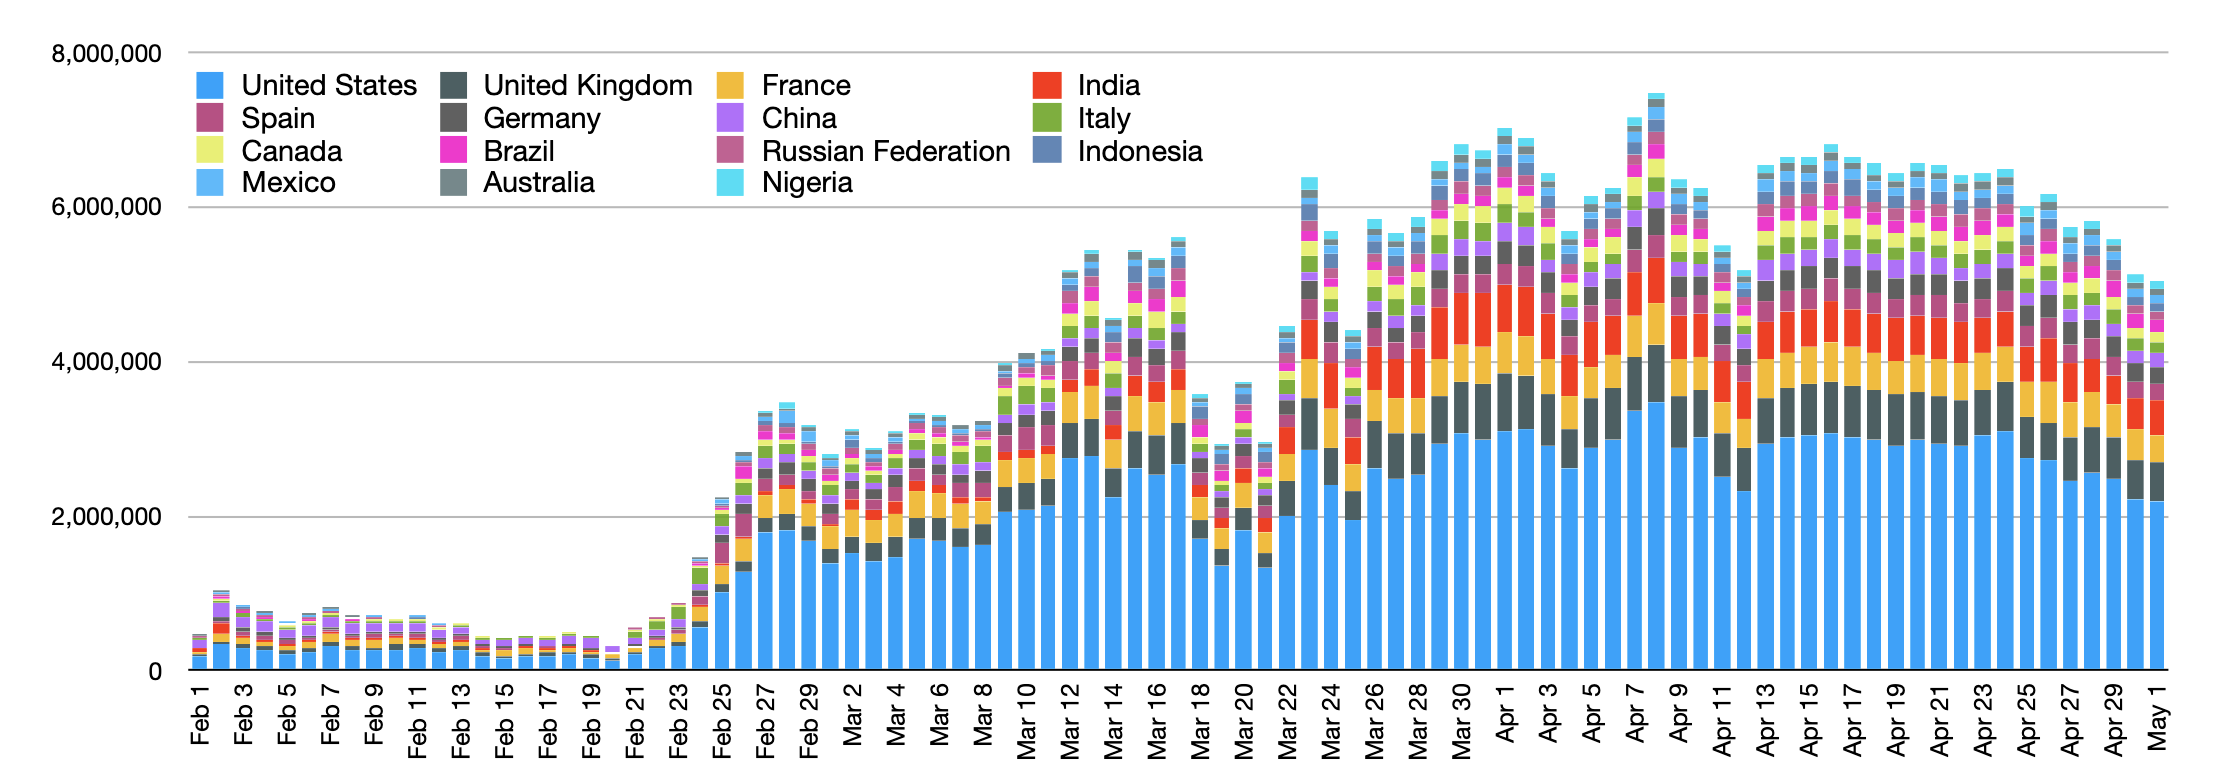
\includegraphics[width=0.8\textwidth]{figs/GeoCov-countrydistribution.png}    
    \centering
    \caption{Daily distribution by country of GeoCoV19 tweets, Feb 1st to May 1st, 2020 \parencite{qaziGeoCoV19DatasetHundreds2020a}}
\end{figure}
%give exact figure instead of 150k here
%https://www.kaggle.com/andradaolteanu/covid-19-sentiment-analysis-social-networks very cool and could be useful!
Of the final dataset, around 150,000 have exact geolocation embedded in the tweet. This is due to the fact that geo-tagging is an explicit option that needs to be set for each tweet, involving activating location data on the mobile app. Another option for geo-tagging is to select a place from a search box; yielding a `place' in the metadata. Both of these types of metadata involve accurate locations, but make up a small proportion of the total geolocated tweets. A third method of geolocating tweets is used to identify most of the locations: when activating a Twitter account the user is strongly encouraged to set their location in their profile. Although it is a free field (generated Place suggestions are included, but are optional), most users set this to their current location; this metadata is included with every tweet. The maintainers of the dataset then employ a toponym extraction approach to elicit the location of the location field. The text of the user location field is first cleaned of non-text characters and symbols. Candidates are then created from the remaining unigrams (single words) and bigrams (pairs of adjacent words), ensuring that two-word place names like `Los Angeles' are included. Groups of three or more words are not considered. Each remaining candidate is filtered against a list of stopwords (see section \ref{textan}), and against the `World Cities Database'\footnote{Available at \texttt{https://www.kaggle.com/max-mind/world-cities-database?select=worldcitiespop.csv}}, an index of 3.1 million worldwide place names, covering 141,989 locations in the US. The remaining candidates are sent as one query to Nominatim, the OpenStreetMap search engine, yielding a best-attempt geolocation: the procedure works best when state and place name is given. Cross-checking the procedure with GPS-geolocated tweets, the dataset shows good coverage and accuracy across US counties, and so makes a panel approach viable. The maintainers of the dataset also presented locations derived from the text of the tweet itself using the same procedure, but we filter these tweets out of the final dataset due to low accuracy. A drawback to this gazeteer approach is that, since users can set their profile location freely, users from other countries or states could masquerade as Americans in particular locations, or the classification process could mis-classify a foreign (particularly English) place as a US location due to sharing a name -- for example, York County, Maine. In order to account for this we remove counties from consideration that have a share of total tweets significantly higher than their population share of the US: Earth, Texas, is the most prominent example of this. Other than misclassification, deliberate setting of the profile location to a US location is possible. This may be a concern for large, well-known cities like Los Angeles and New York, but it is less likely that a given user will set their location to a less well-known American county. Finally, users may move county and not change their location.
\begin{figure}[h!]
    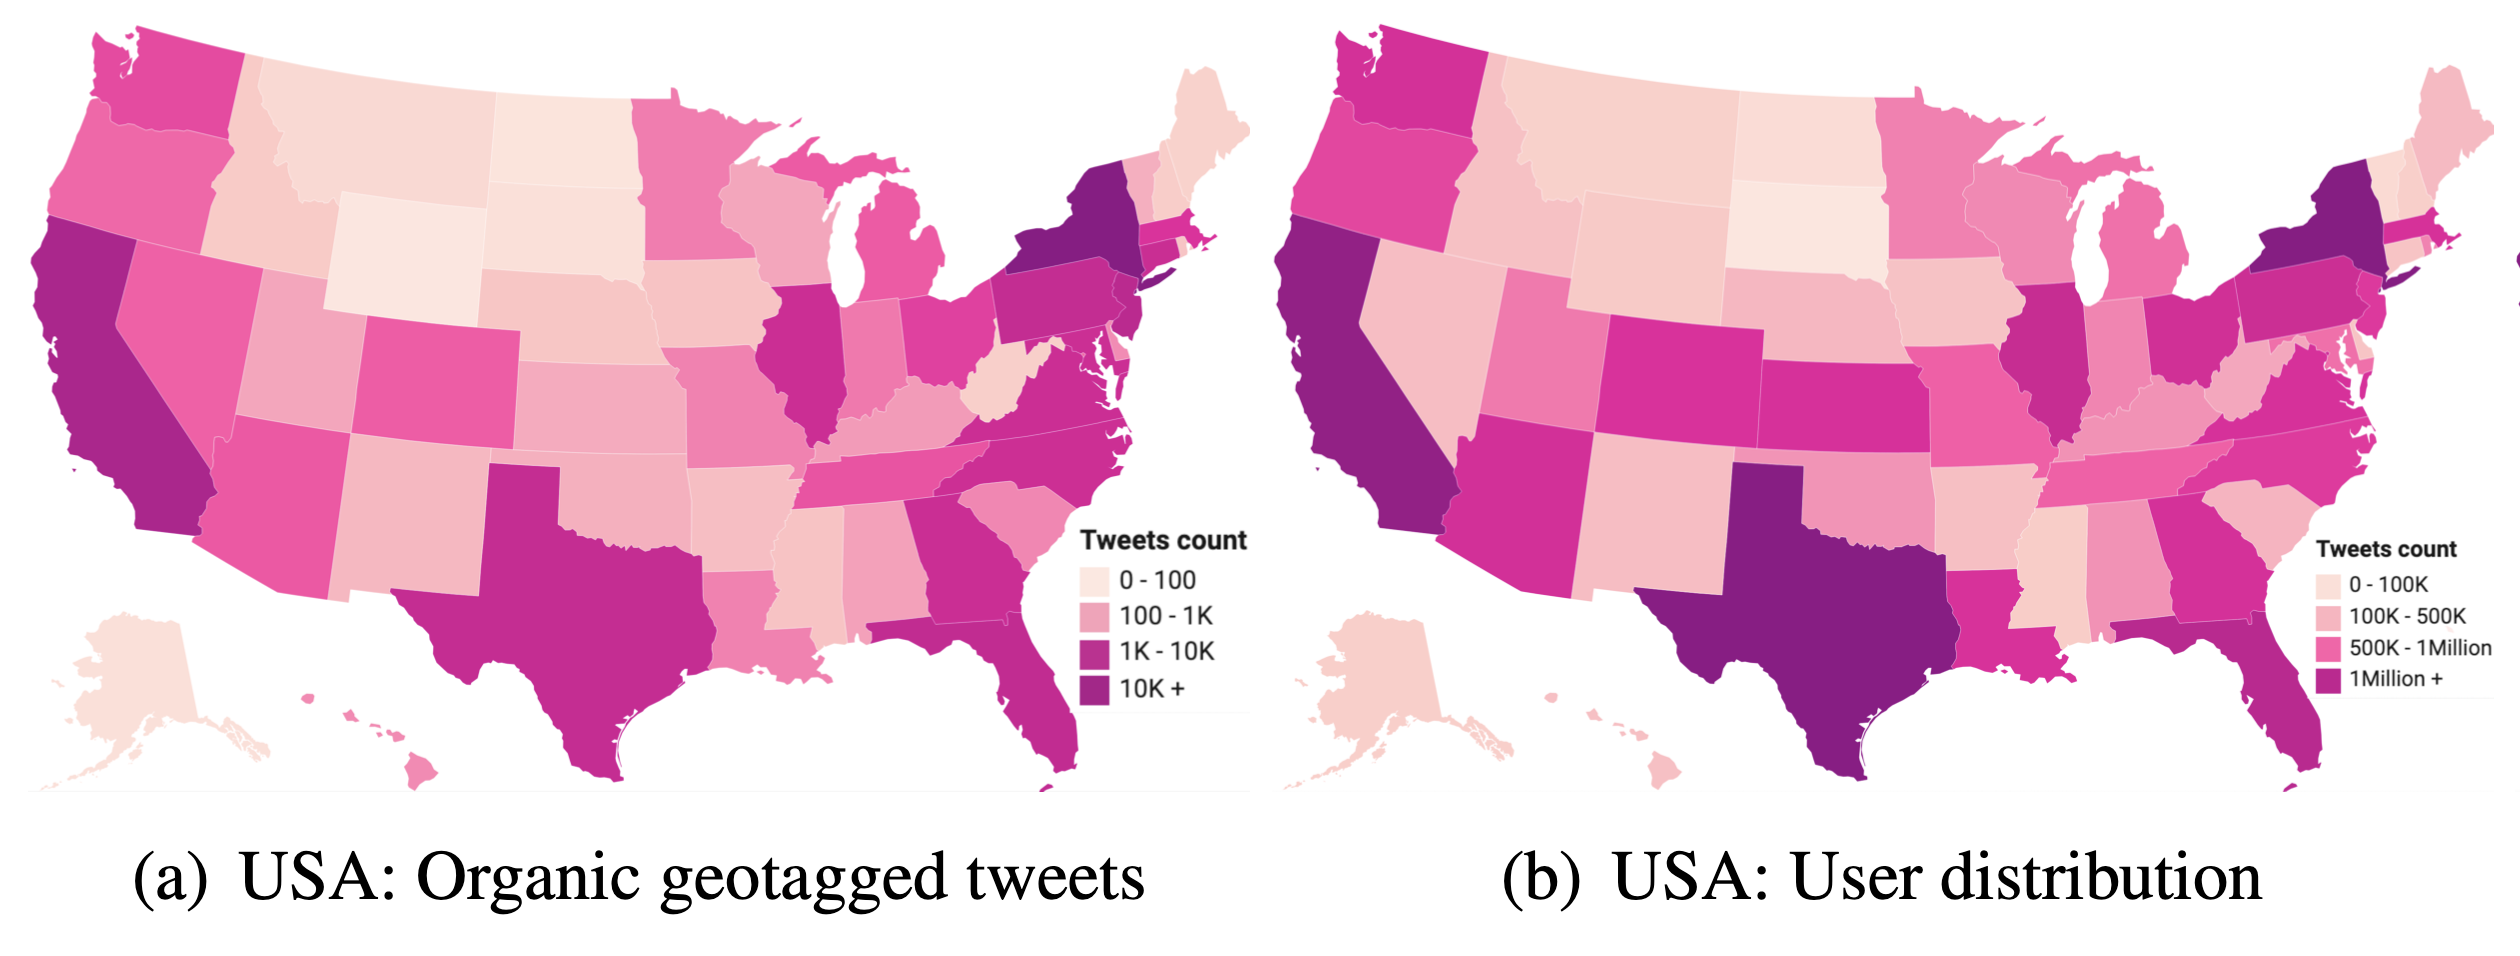
\includegraphics[width=0.8\textwidth]{figs/GeoCov-USdist.png}    
    \centering
    \caption{Geographic distribution of GeoCoV19 tweets and users \parencite{qaziGeoCoV19DatasetHundreds2020a}}
\end{figure}

Twitter's terms of service restrict the large-scale sharing of Tweet datasets; hence public-facing tweet datasets can only be made available `dehydrated', with only the universal identifiers (a long number that maps to the tweet in Twitter's database) given, instead of the tweet text and assorted metadata. In order to use the dataset to analyse tweet content, researchers wishing to use the dataset must apply and be accepted for a Developer account. This gives access to a password called an API key, which is used to query the Twitter API with the identifiers to `rehydrate' and gain access to the full tweet text and metadata. Since the tweets are delivered from the servers at download time, this procedure entails that a proportion of Tweets -- those identified as containing misinformation or those sent by users whose accounts have since been suspended or deleted -- will be unavailable on request from the service when the dataset is `rehydrated'. This presents a selection problem for topics like misinformation, where Twitter enacts a stringent and continuous policy. A prominent concern for my data might be the suspension of Donald Trump's prolific Twitter account; his tweets were a touchstone for right-wing US online conversations. This does not present an issue to my data, however, because tweets interacting with tweets from a deleted account are still available from the API. The deletion rate ultimately encountered during the rehydration process was around 20\%, reflecting the normal removal of machine-generated content.


\section{Methods}%4000 words
\subsection{Text analysis}\label{textan}


\section{Results}%1000 words

\section{Discussion} %1000 words

\wordcount
\printbibliography

\end{document}